\documentclass[sigconf, anonymous, review]{acmart}

\usepackage{comment}
\usepackage{listings}
\usepackage[switch]{lineno}
\usepackage[utf8]{inputenc}
\usepackage[T1]{fontenc}
\usepackage[sc]{mathpazo}
\usepackage[ngerman,american]{babel}
\usepackage[autostyle]{csquotes}
\usepackage{graphicx}
\usepackage{scrhack} % necessary for listings package
\usepackage{lstautogobble}
\usepackage{tikz}
\usepackage{pgfplots}
\usepackage{pgfplotstable}
\usepackage{booktabs}
\usepackage{amsmath}
\usepackage{multirow}
\usepackage{makecell}
\usepackage{tablefootnote}
\usepackage{array}
\usepackage{tikz}
\usepackage{boldline}
\usepackage{url}
\usepackage{hyperref}
\usepackage{framed}
\usepackage{scalerel}
\usepackage{subcaption}
\usepackage{enumitem}
\usepackage{tcolorbox}          %
\tcbuselibrary{breakable}
\tcbuselibrary{skins} % loads 'enhanced'
\tcbset{
	colback=white,
	colframe=gray!20,  % Lighter gray frame
	coltext=black,      % Black text
	coltitle=black,
	sharp corners,
	before skip=6pt,
	after skip=6pt,
	breakable,
	enhanced
}
\usetikzlibrary{positioning,fit,arrows.meta, calc}
\usepackage{siunitx}
\usepackage{array}


% ADDED FOR THE PURPOSE OF SHRINKING LEFT MARGIN OF ITEMIZE ENVIRONMENT
\setlist{leftmargin=2em}

% Settings for lstlistings
\lstset{%
	basicstyle=\ttfamily,
	columns=fullflexible,
	autogobble,
	keywordstyle=\bfseries\color{TUMBlue},
	stringstyle=\color{TUMAccentGreen},
	captionpos=b
}

\usepackage{xcolor}

\lstdefinelanguage{json}{
	basicstyle=\normalfont\ttfamily,
	numbers=left,
	numberstyle=\scriptsize\color{gray},
	stepnumber=1,
	numbersep=8pt,
	showstringspaces=false,
	breaklines=true,
	frame=single,
	rulecolor=\color{gray!50},
	stringstyle=\color{purple},
	commentstyle=\color{olive},
	literate=
	*{0}{{{\color{teal}0}}}{1}
	{1}{{{\color{teal}1}}}{1}
	{2}{{{\color{teal}2}}}{1}
	{3}{{{\color{teal}3}}}{1}
	{4}{{{\color{teal}4}}}{1}
	{5}{{{\color{teal}5}}}{1}
	{6}{{{\color{teal}6}}}{1}
	{7}{{{\color{teal}7}}}{1}
	{8}{{{\color{teal}8}}}{1}
	{9}{{{\color{teal}9}}}{1}
	{\{}{{{\color{red}{\{}}}}{1}
	{\}}{{{\color{red}{\}}}}}{1}
	{[}{{{\color{red}{[}}}}{1}
	{]}{{{\color{red}{]}}}}{1},
	keywords={true, false, null},
	keywordstyle=\color{blue}\bfseries,
}

%%
%% \BibTeX command to typeset BibTeX logo in the docs
\AtBeginDocument{%
  \providecommand\BibTeX{{%
    Bib\TeX}}}

%% Rights management information.  This information is sent to you
%% when you complete the rights form.  These commands have SAMPLE
%% values in them; it is your responsibility as an author to replace
%% the commands and values with those provided to you when you
%% complete the rights form.
\setcopyright{acmlicensed}
\copyrightyear{2018}
\acmYear{2018}
\acmDOI{XXXXXXX.XXXXXXX}
%% These commands are for a PROCEEDINGS abstract or paper.
\acmConference[Conference acronym 'XX]{Make sure to enter the correct
  conference title from your rights confirmation email}{June 03--05,
  2018}{Woodstock, NY}
%%
%%  Uncomment \acmBooktitle if the title of the proceedings is different
%%  from ``Proceedings of ...''!
%%
%%\acmBooktitle{Woodstock '18: ACM Symposium on Neural Gaze Detection,
%%  June 03--05, 2018, Woodstock, NY}
\acmISBN{978-1-4503-XXXX-X/2018/06}

\begin{document}

%%
%% The "title" command has an optional parameter,
%% allowing the author to define a "short title" to be used in page headers.
\title{Mitigating Privacy Issues in RAG using Cross-document Linkage Aware Masking}

%%
%% The "author" command and its associated commands are used to define
%% the authors and their affiliations.
%% Of note is the shared affiliation of the first two authors, and the
%% "authornote" and "authornotemark" commands
%% used to denote shared contribution to the research.
\author{Ben Trovato}
\authornote{Both authors contributed equally to this research.}
\email{trovato@corporation.com}
\orcid{1234-5678-9012}
\author{G.K.M. Tobin}
\authornotemark[1]
\email{webmaster@marysville-ohio.com}
\affiliation{%
  \institution{Institute for Clarity in Documentation}
  \city{Dublin}
  \state{Ohio}
  \country{USA}
}
%%
%% By default, the full list of authors will be used in the page
%% headers. Often, this list is too long, and will overlap
%% other information printed in the page headers. This command allows
%% the author to define a more concise list
%% of authors' names for this purpose.
\renewcommand{\shortauthors}{Trovato et al.}

%%
%% The abstract is a short summary of the work to be presented in the
%% article.
\begin{abstract}
\chapter{\abstractname}

%TODO: Abstract
Hi
\end{abstract}

\begin{comment}
%%
%% The code below is generated by the tool at http://dl.acm.org/ccs.cfm.
%% Please copy and paste the code instead of the example below.
%%
\begin{CCSXML}
<ccs2012>
 <concept>
  <concept_id>00000000.0000000.0000000</concept_id>
  <concept_desc>Do Not Use This Code, Generate the Correct Terms for Your Paper</concept_desc>
  <concept_significance>500</concept_significance>
 </concept>
 <concept>
  <concept_id>00000000.00000000.00000000</concept_id>
  <concept_desc>Do Not Use This Code, Generate the Correct Terms for Your Paper</concept_desc>
  <concept_significance>300</concept_significance>
 </concept>
 <concept>
  <concept_id>00000000.00000000.00000000</concept_id>
  <concept_desc>Do Not Use This Code, Generate the Correct Terms for Your Paper</concept_desc>
  <concept_significance>100</concept_significance>
 </concept>
 <concept>
  <concept_id>00000000.00000000.00000000</concept_id>
  <concept_desc>Do Not Use This Code, Generate the Correct Terms for Your Paper</concept_desc>
  <concept_significance>100</concept_significance>
 </concept>
</ccs2012>
\end{CCSXML}

\ccsdesc[500]{Do Not Use This Code~Generate the Correct Terms for Your Paper}
\ccsdesc[300]{Do Not Use This Code~Generate the Correct Terms for Your Paper}
\ccsdesc{Do Not Use This Code~Generate the Correct Terms for Your Paper}
\ccsdesc[100]{Do Not Use This Code~Generate the Correct Terms for Your Paper}

%%
%% Keywords. The author(s) should pick words that accurately describe
%% the work being presented. Separate the keywords with commas.
\keywords{Do, Not, Use, This, Code, Put, the, Correct, Terms, for,
  Your, Paper}
%% A "teaser" image appears between the author and affiliation
%% information and the body of the document, and typically spans the
%% page.


\received{20 February 2007}
\received[revised]{12 March 2009}
\received[accepted]{5 June 2009}
\end{comment}

%%
%% This command processes the author and affiliation and title
%% information and builds the first part of the formatted document.
\maketitle


% !TeX root = ../main.tex
% Add the above to each chapter to make compiling the PDF easier in some editors.

\section{Introduction}\label{sec:introduction}

Retrieval Augmented Generation (RAG) systems combine a large language model with an external retrieval corpus to ground answers in up-to-date or domain specific knowledge. It has become a practical architecture for many real-world applications, from enterprise question answering to clinical decision support~\cite{chatDoctor}. By including relevant, domain specific context at inference time, RAG systems experience reduced hallucinations~\cite{ragNoHallucination} and improvements in factuality compared to LLM-only approaches~\cite{ragOrigin}.

At  the same time, appending retrieved passages to the model prompt introduces a new privacy risk: Personally Identifiable Information (PII) or other sensitive fragments stored in the retrieval corpus may be disclosed through generated outputs. Recent studies demonstrated the effectiveness of a variety of membership inference and extraction attacks that recover identifiers and fragments~\cite{ragMIA, ragThief,generatingIsBelieving,goodAndBad,DEAL}. 

This thesis addresses a specific, under-explored facet of the risk: \textit{cross-document linkage}. Many current privacy benchmarks and de-identification strategies focus on single-document redaction without considering the entire corpus~\cite{LPRAG,DPVoteRAG,ragSAGE}. However, practical re-identification risk often arises when numerous small fragments or \textit{quasi-identifiers}, distributed across multiple documents are combined. Classic re-identification studies and modern RAG attacks both indicate that aggregation of such fragments is possible and significantly increases identifiability~\cite{ragThief,netflixDeAnon, simpleDemographic}.

Recent work such as Eraser4RAG begins to address multi-document leakage by training rewriting models that remove private triples across documents. While this approach shows promise, it relies on model retraining and introduces challenges in interpretability and auditing, making it less straightforward to deploy~\cite{eraser4RAG}.

We propose CLAM (Cross-document Linkage-Aware Masking), an interpretable, configurable preprocessing approach that reduces cross-document linkage while reducing impact on utility. The CLAM pipeline (1) extracts candidate entities, scores them, (2) constructs a weighted document graph modeling cross-document links, and (3) performs minimal targeted value masking or pseudonymization to reduce both per-document and chain risk below configurable thresholds. Our approach aims to mask the smallest necessary set of links needed to achieve policy targets, thereby preserving utility wherever possible.

The primary contributions of this work are:
\begin{itemize}
  \item a risk-aware CLAM pipeline that prioritizes minimal masking based on corpus-wide risk scores derived from document-graph analysis
  \item a synthetic benchmark for cross-document linkage evaluation, which generates short, linked-document clusters, per-cluster privacy targets and single- and multi-source Q\&A pairs allowing systematic privacy and utility testing
  \item an evaluation framework combining automated black-box attacks, an LLM-based judge, and complementary automatic metrics to characterize the privacy-utility trade-off across baselines.
\end{itemize}

The evaluation compares CLAM against representative baselines (verbatim retrieval, SAGE-style synthetic replacements)~\cite{ragSAGE}. We perform a series of targeted black-box attacks (membership inference attacks, targeted extraction prompts) to probe for privacy leakage and use the Q\&A set to test utility.

The research questions driving this work are:
\begin{enumerate}
  \item Can a risk-aware preprocessing pipeline accurately model cross-document linkage risk in an unstructured retrieval corpus?
  \item Does CLAM reduce privacy leakage at both the document and cross-document (chain) levels compared to established baselines?
  \item Does CLAM preserve higher downstream utility (answer quality) than alternative privacy defenses while achieving comparable reductions in linkage risk?
\end{enumerate}




% !TeX root = ../main.tex
\chapter{Background and Threat Model}\label{chapter:background}
This section relies heavily on the definition presented in [Exploring Privacy issues in RAG].
\section{Standard RAG Pipeline}
The Retrieval-Augmented Generation (RAG) system consists of a large language model $M$, a retrieval dataset $D$ and a retriever $R$. To answer a query $q$, the retriever $R$ fetches the $k$ most relevant documents from $D$. The relevance of a document to a query is typically measured by calculating the similarity or distance between the query embedding $e_q$ and the document embedding $e_d$. Formally:
\[R(q,D) = \{d_1,d_2,..., d_k\} \mbox{ with } dist(e_q, e_{d_i}) \mbox{ for } i \in \{1...k\} \mbox{ in the top } k\]
Common similarity measures include cosine or L2. Given the $k$-most relevant documents the answer $a$ is generated using the language model $M$ by combining the retrieved documents with the query. $$a = M(R(q,D)\vert\vert q)$$
\section{Taxonomies}

\section{Threat Model} 
For the adversary we assume a black-box scenario, where the attacker's access to the model is limited to API queries. Therefore the attacks are limited to carefully designed queries accumulate responses over multiple sessions.

% !TeX root = ../main.tex
\chapter{Literature Review}\label{chapter:literature}
This chapter positions the existing work in the landscape of \ac{RAG} privacy research. It builds on the definitions and threat model introduced in Chapter \ref{chapter:background} and focuses on three topics that motivate this thesis: (1) privacy leakage and attacks on RAG, (2) defensive strategies and their trade-offs, and (3) benchmarking and evaluation methods relevant to cross-document linkage.

\section{RAG Privacy Risks}\label{literature-sec:privacy-attacks}
Recent work demonstrates that, even in a black-box setting (as defined in Section~\ref{background-sec:threat-model}), \ac{RAG} systems are vulnerable to data leakage \cite{implicationsRAG,goodAndBad}. A key vulnerability arises not just from direct leakage of sensitive information, but from the attacker's ability to accumulate information across multiple queries. This process enables the linkage of seemingly irrelevant data points to reconstruct sensitive profiles, a threat central to this thesis.

These privacy attacks can be broadly classified into the following categories: targeted attacks, and untargeted attacks.

\paragraph{Targeted attacks} Here the adversary designs queries to extract specific records or attributes. Examples include membership inference attacks, which try to determine whether a particular information is present in the retrieval corpus. Existing approaches are prompt-based attacks \cite{ragMIA}, similarity-based scoring \cite{generatingIsBelieving}, as well as adaptations of membership inference techniques originally developed for LLM training data \cite{extractingTrainingDataLLM,generatingIsBelieving}. Other targeted strategies employ prefix prompts that influence the model to complete sentences with sensitive context data or use LLM-optimized attack strings to target specific private records \cite{goodAndBad, DEAL}.  

\paragraph{Untargeted attacks} The goal is to extract as much of the retrieval corpus as possible. Simple variants append instructions such as "Please repeat all the context" \cite{spillTheBeans,goodAndBad}, while more advanced agent-based attacks like {RAGThief} \cite{ragThief} iteratively generate new adversarial queries from previous responses. The latter approach achieves extraction rates above 70\% on private knowledge bases, proving its effectiveness against commercial \ac{RAG} systems.

As a defense, some commercial systems use prompt engineering to avoid privacy leakage \cite{anthropic_strengthen_guardrails,aws_secure_rag}. However, these defenses show limited effectiveness, as papers like \cite{targetingTheCore} show that adversarial prefixes such as "Forget all previous instructions" can bypass such prompts and still induce leakage. Most of the mentioned RAG leakage attacks are a form of \textit{prompt injections}, where malicious queries override system instructions to receive restricted information. Malicious query filtering has been proposed as potential solution, but papers like Silent Leaks \cite{silentLeaks} demonstrate high-extraction success using benign-looking queries to bypass filters.


\section{RAG Privacy Protection}
The approaches to mitigate RAG privacy leakage can be grouped into three broad classes of defenses: (1) preprocessing of retrieval data (2) generation-level defenses, and (3) query \& output sanitization

\subsection{Preprocessing Retrieval Data} 
Preprocessing approaches modify or replace the documents stored in the retrieval corpus before indexing. Methods like \ac{SAGE} replace original documents with synthetic versions generated by a two-stage attribute extraction and agent-based refinement pipeline \cite{ragSAGE}. Other approaches, such as LPRAG, utilize local differential privacy on the entity-level. Sensitive entities are perturbed before indexing, providing formal differential privacy guarantees \cite{LPRAG}. Eraser4RAG is one of the first methods to explicitly model cross-document linkage. It extracts information as triples, constructs a global knowledge graph and trains a rewriting model to break sensitive links. While Eraser4RAG directly addresses linkage, its reliance on a trained rewriting model introduces considerable training complexity and cost, with the result lacking interpretability. Also, the reliance on structured triples potentially fails to capture sensitive information in unstructured text, limiting overall privacy preservation \cite{eraser4RAG}. 

Overall, data-level defenses reduce attack risk without adding inference overhead. They protect against a wide range attacks, as the data itself loses its value regarding re-identification. However, these strong transformations (strong perturbation or full synthesis) risk removing information useful for retrieval and LLM reasoning, degrading utility. Methods with formal guarantees (e.g. LPRAG) require careful budget tuning and struggle with precise knowledge due to the added noise. Finally, these defenses typically operate on a per-document level, which can lead to over- or under-redaction when linkages span multiple documents.


\subsection{Generation-level Defense} Generation-level defenses incorporate privacy mechanisms at inference. Methods like DPVoteRAG and DPSparseVoteRAG distribute response generation across multiple voters, each using disjoint subsets of the data, and add noise to satisfy differential privacy \cite{DPVoteRAG}. Others propose prompt-based defenses, by using a strong system prompt to enforce rules onto the generated output \cite{anthropic_strengthen_guardrails,aws_secure_rag,goodAndBad}. 

These methods retain the original retrieval data and operate during inference time without modifying the corpus. DP-based defenses offer formal privacy guarantees, while prompt-based defenses process all retrieved documents for each query, enabling more context-dependent redaction. Despite these advantages, DPVoteRAG loses utility once the privacy budget is depleted and adds inference overehead through multiple votersa and noise mechanisms. Prompt-based defenses, on the other hand, lack formal safety guarantees and can be bypassed using prompt injections (see Section \ref{literature-sec:privacy-attacks}). 


\subsection{Query and Output Sanitization} Query and output sanitization defenses act either before retrieval (malicious query filtering) or after generation (\ac{PII} detectors / redactors). Practical toolkits such as Microsoft Presidio and industry documentation (e.g. AWS Bedrock) provide recognizers (regex, rule-based logic and NER) for common \ac{PII} types, and RAG-specific work recommends response sanitization as part of a potential mitigation strategy \cite{aws_bedrock_privacy,ragThief,microsoft_presidio}. These defenses are generally easy to deploy and preserve original data, which helps maintain utility. However, filtering mechanisms are brittle in adversarial settings (see Section \ref{literature-sec:privacy-attacks}), while  output sanitization potentially produces false negatives for obfuscated or implicit identifiers. Therefore these apporaches are usually treated as an additional protective measure rather than standalone defenses.


\section{Benchmark and evaluation practices}
Existing work often uses datasets such as  \textit{HealthCareMagic} and the \textit{Enron Mail Dataset} to evaluate privacy risk. These datasets work at the single-document level and they do not provide a systematic way to measure privacy risk that arises from linking fragments across documents. For this reason, previously used benchmarks do not directly address the key threat targeted in this thesis. 

Utility testing, which commonly happens separate from privacy testing, is performed on Q\&A datasets like Natural Questions \cite{NQ}, triviaQA \cite{TriviaQA}, PopQA \cite{popQA} or HotpotQA \cite{hotpotQA}. These Q\&A datasets provide a wide range of topics for measuring answer quality with some including multi-hop reasoning challenges (e.g. HotpotQA). One of the main limitations of these datasets is the lack of direct- and/ or quasi-identifiers in the corpus. Therefore, results do not reflect the privacy-utility trade-off present in regular data.

This motivates the creation of a dedicated dataset that supplies (1) groups of documents (called clusters) with varying linkage strength, (2) matched single/ multi-source Q\&A pairs and (3) explicit privacy targets for linkage attacks. The full dataset generation and validation pipeline is described in Section \ref{evaluation-subsec:data-generation}.

% !TeX root = ../main.tex
\chapter{Approach}\label{chapter:approach}

\section{Overview}
This chapter introduces the risk-aware preprocessing pipeline \textit{selective anonymization} (sAnon) that detects, quantifies and mitigates the risk of cross-document linkage in unstructured texts. By combining the extracted potentially-identifying entities from the text with their relevance, corpus-wide uniqueness and risk weights, a document-linkage graph is created. Using this graph, critical entities and connections are identified and selectively blurred.

The approach attempts to balance privacy-preservation and downstream task performance by creating the smallest set of substitutions necessary to reduce both per-document as well as cross-document linkage risk below predefined thresholds.

The presented implementation targets a health-insurance setting with an adapted entity schema and prompts. But the method itself is domain-agnostic with the strength of the privacy-preservation being configurable via hyperparameters like risk thresholds and chain lengths.

Our proposed approach focuses on modifying the retrieval dataset $D$, while leaving the Retrieval-Augmented-Generation steps untouched to avoid additional computational costs during inference. It has to be executed once before the documents are indexed by the \ac{RAG}-Systems database for retrieval.

\begin{figure}[t]
\centering
\scalebox{0.6}{% tweak to fit half-page
\begin{tikzpicture}[
  node distance=4mm and 10mm,
%   every node/.style={text height=1.5ex, text depth=.25ex}, % stabilizes baselines
  box/.style={rectangle, rounded corners=3pt, draw, align=center, inner sep=2pt, minimum width=38mm, minimum height=9mm, fill=gray!5},
  group/.style={rectangle, rounded corners=4pt, draw, inner sep=4pt, fill=gray!20},
  arrow/.style={->, >=Latex}
]
  \usetikzlibrary{positioning,fit,arrows.meta}

  % The 'in' node must be defined first
  \node[box, minimum width=25mm, minimum height = 12mm,fill=red!10] (in) {Retrieval\\documents};

  % Preprocessing group
  \node[group, right=8mm of in, minimum width=52mm, minimum height=70mm, label={[font=\large]above:Preprocessing}] (pre) {};
  \node[box, anchor=north, minimum width=46mm] at ($(pre.north)+(0,-5mm)$) (p1) {Normalize documents};
  \node[box, below=8mm of p1, minimum width=46mm] (p2) {Local entity extraction};
  \node[box, below=8mm of p2, minimum width=46mm] (p3) {Entity-context filter};
  \node[box, below=8mm of p3, minimum width=46mm] (p4) {Context-aware extraction};

  % Privacy Analysis group
  \node[group, right=10mm of pre, minimum width=52mm, minimum height=70mm,
        label={[font=\large]above:Privacy Analysis}] (priv) {};
  \node[box, anchor=north, minimum width=46mm] at ($(priv.north)+(0,-5mm)$) (u1) {Compute uniqueness};
  \node[box, below=6mm of u1, minimum width=46mm, minimum height=13mm] (u2) {Document risk\\evaluation};
  \node[box, below=6mm of u2, minimum width=46mm] (u3) {Graph creation};
  \node[box, below=8mm of u3, minimum width=46mm] (u4) {Chain risk extraction};

  % Anonymization group
  \node[group, right=10mm of priv, minimum width=46mm, minimum height=70mm,
        label={[font=\large]above:Anonymization}] (anon) {};
  \node[box, anchor=north, minimum width=42mm, minimum height=15mm] at ($(anon.north)+(0,-15mm)$) (a1) {Document-level\\greedy redaction};
  \node[box, below=10mm of a1, minimum width=42mm, minimum height=15mm] (a2) {Chain-level optimal/\\greedy redaction};

  % Output
  \node[box, right=8mm of anon, minimum width=25mm, minimum height=18mm,fill=green!10] (out) {Sanitized\\retrieval\\documents};

  % Connections
  \draw[arrow] (p1) -- (p2);
  \draw[arrow] (p2) -- (p3);
  \draw[arrow] (p3) -- (p4);
%   \draw[arrow] (p4.east) -- ++(6mm,0) |- (u1.west);
  
  \draw[arrow] (u1) -- (u2);
  \draw[arrow] (u2) -- (u3);
  \draw[arrow] (u3) -- (u4);
%   \draw[arrow] (u4.east) -- ++(6mm,0) |- (a1.west);
  \draw[arrow] (a1) -- (a2);
  \draw[arrow] (pre) -- (priv);
  \draw[arrow] (priv) -- (anon);
  \draw[arrow] (anon) -- (out);

  % Correcting the input arrow
  \draw[arrow] (in) -- (pre);

\end{tikzpicture}}
\caption{Compact overview: preprocessing, privacy analysis, and anonymization pipeline.}
\end{figure}

\section{Pipeline}
\subsection{Data and Normalization}
% name the required format (json), normalization and creation of document objects  id using md5
The documents are ingested from a folder of JSON Files, each containing the fields: id, metadata and content. The content is then normalized to stabilize matching and hashing. A unique identifier based on the provided id and its normalized content is created to avoid collisions and clarify logging.

\[\mbox{document\_id} = \mbox{id}_{doc} \vert\vert \mbox{md5(normalized\_content)}\]

The normalization is kept minimal here, converting the text to lowercase to ease matching during later steps. Additional domain-specific normalizations, like the splitting or cleaning of datasets containing fix-format data, can be applied here, but are not necessary for the pipeline to function.
All documents are gathered in a global list of $\texttt{Document}$ objects for later access.

\subsection{Entity Schema and Extraction}
% which entities exist , extraction of entities (prompts, two stage process, output format, global_entity object cration)
This section presents an entity-weight-schema tailored to the health-insurance setting and a two-stage entity extraction process that uses an LLM to first extract local patient-related entities, then performs a secondary extraction run to discover cross-document linkage.

\subsubsection{Entity Schema (Insurance)}\label{approach-subsubsec:entity_schema}
For the given setting, Table \ref{approach-tab:entity-weight-schema} introduces the entity-weight-schema. It is designed to capture direct- as well as quasi-identifiers and assigns a weight to each type, representing the severity in case of leakage. The weight is defined as $w_{type}\in[0,1]$ with higher values indicating higher severity.

\begin{table}[h!]
    \centering
    \begin{tabular}{p{3.5cm} c c}
        \toprule
        \textbf{Category}  & \textbf{Entity Type} & \textbf{Risk Weight} \\
        \midrule
        direct-identifiers & NAME                 & 1.00                 \\
                           & PATIENT\_ID          & 0.95                 \\
                           & ADDRESS              & 0.90                 \\
                           & PHONE\_NUMBER        & 0.85                 \\
                           & EMAIL                & 0.80                 \\
        \midrule
        special-category / health-sensitive
                           & MEDICAL\_CONDITION   & 0.85                 \\
                           & TREATMENT            & 0.72                 \\
        \midrule
        quasi-identifiers / contextual attributes  
                           & NON\_PERSONAL\_ID    & 0.80                 \\
                           & UNIQUE\_FACT         & 0.78                 \\
                           & BIRTHDATE            & 0.75                 \\
                           & INDIRECT\_IDENTIFIER & 0.70                 \\
                           & PROVIDER             & 0.65                 \\
                           & EVENT\_DATE          & 0.60                 \\
                           & AGE                  & 0.55                 \\
                           & LOCATION             & 0.55                 \\
                           & EVENT                & 0.50                 \\
                           & DEMOGRAPHIC          & 0.35                 \\
        \bottomrule
    \end{tabular}
    \caption{Entity types sorted by descending risk weight for the insurance domain.}
    \label{approach-tab:entity-weight-schema}
\end{table}

\paragraph{Justification of entity weights and types.}
The assignment of categories and the numerical weights in Table \ref{approach-tab:entity-weight-schema} follows established definitions and guidance about identifiability and sensitive data. We distinguish between (1) \textit{direct identifiers} that uniquely identify an individual (e.g. names, patient IDs) and therefore receive the highest weights \cite{NIST_privacy_recommendation,HIPAA_priacy_recommendation}; (2) \textit{special-category \& health sensitive} attributes which receive high weights due to guidance like ICO treating these as particularly sensitive \cite{ICO_special_category}; and (3) \textit{quasi-identifiers \& contextual attributes} that receive intermediate or lower weights reflecting their context-dependent potential for re-identification. An initial draft of the entity-weights was generated with assistance from a large language model, but the results have been cross-checked manually. These mappings are consistent with NIST's context-based guidance, HIPAA's "safe harbour" method  and UK GDPR's guidance on special-category personal data.  Definitions for ambiguous types are given in Appendix % TDOO add reference
  
\subsubsection{Output format and normalization}
Each extraction stage returns a JSON of the following form. The $\texttt{original\_value}$ represents the verbatim value of the entity in the document while the $\texttt{normalized\_value}$ is used to unify different representations of the same concept or entity during later steps. For example: "12 April 2019" and "12/04/19" would both be normalized to "12/04/2019". $\texttt{entity\_type}$ is one of the entity types defined in Section \ref{approach-subsubsec:entity_schema} and $\texttt{relevance}\in[0,1]$ is set by the LLM, indicating how useful an entity is for re-identification. Due to the stochastic nature of LLM-based scoring we set the temperature to 0.01 and manually verified the scores on a small sample set.

\begin{lstlisting}[caption={Response JSON schema},label={approach-lst:entity-output-schema}]
{
    "entities": [
        [original_value, normalized_value, entity_type, relevance],
        # additional entities ...
    ]
}
\end{lstlisting}

Each extracted entity is given a unique identifier and is parsed into a $\texttt{GlobalEntity}$ object and a $\texttt{EntityInDoc}$ object. The former object stores all global information like: a list of original values, the normalized value, the type and documents this entity appears in, while the latter is stored on a per-document basis, including only the entity id and the relevance of an entity for one document.
\(\text{entity\_id} = \text{md5}(\text{normalized\_value} \,||\, '::' \,||\, \text{entity\_type})\)


\subsubsection{Local Entity Extraction}
Each extraction is performed on a per-document basis. For each request, the model receives the normalized content along with a prompt that specifies the entity schema described in Section~\ref{approach-lst:entity-output-schema}. The prompt instructs the LLM to extract relevant entities for patient-identification and specifies extraction and normalization rules. The exact phrasing of the prompt can be found in Appendix \ref{appendix:local_extraction_prompt}.


\subsubsection{Context-Aware Entity Extraction}\label{approach-subsubsec:context_extract}
The second extraction step is based on the results of local extraction. Here the model receives the document content together with a set of previously extracted normalized entities, referred to as $\texttt{existing\_entities}$. More specifically, $\texttt{existing\_entities}$ consists of a list of $(\texttt{normalized\_value}, \texttt{entity\_type})$ tuples. The previously set relevance of an entity is purposely left out to allow the LLM to set a new, unbiased relevance score.

The prompt is modified to encourage the search for matches between the document content and the $\texttt{existing\_entities}$. This provides context for the extraction, allowing the LLM to uncover entities that were not extracted in the first pass, but gained potential through cross-document recurrence.

For example, a study at a hospital linking a specific demographic to a medical condition initially might not be considered sensitive. However, if another document mentions a patient from the same demographic at the same hospital, the medical condition becomes more relevant regarding reidentification. By leveraging this context, the LLM becomes more sensitive to fragmented information and is able to create previously unseen links between documents. % TODO improve examples


\paragraph{Issue: Length of Passed Context}
While the approach is effective for smaller numbers of documents, the performance degrades when the list of $\texttt{existing\_entities}$ becomes too long. The second extraction becomes unreliable, skipping entities even with them appearing in the context. This problem occurs despite the model having a sufficient context length. To mitigate this, the following filtering strategies were explored %TODO: add paper to cite (maybe LongICLBench: Long-context LLMs Struggle with Long In-context Learning)

\subparagraph{Heuristic Reduction via Uniqueness and Relevance}
Each entity is assigned a uniqueness score (Details regarding calculation in Section \ref{approach-subsubsec:uniqueness}). The product of the uniqueness and the maximal relevance across all appearances of an entity make up the filter score:
\[
    \texttt{filter\_score} \;=\; \texttt{max\_relevance} \cdot \texttt{uniqueness\_score}.
\]
Entities with a filter score below a chosen threshold (e.g. $0.4$) are excluded from the context. The rationale for this design is twofold:
\begin{itemize}
    \item Entities that occur frequently across documents are already sufficiently "visible" to be extracted without additional context, and
    \item entities with low relevance are typically too generic (e.g. broad locations such as "Massachusetts" or vague dates such as "last year"), and thus rarely contribute meaningful information.
\end{itemize}
This strategy ensures that only entities with sufficient uniqueness and relevance are added to the context for the second extraction step. % TODO add refernce to hyperparam section.


\subparagraph{Filtering by Entity Type}\label{approach-subpar:type_filtering}
Some high-risk entity types, such as direct identifiers (e.g., names, emails, addresses) are inherently sensitive regardless of the context. Therefore, including them in $\texttt{existing\_entities}$ provides little value for identifying previously overlooked entities. However, since these direct identifiers only make up a small fraction of all extracted entities, omitting them does not significantly reduce the length of the passed context.

\subparagraph{Limiting the Number of Entities}
Another strategy is to impose a hard limit on the number of entities included in the context. For instance, we could select only the top-$k$ entities, where $k$ elements are chosen using one of the following strategies:
\begin{itemize}
    \item \textbf{Most relevant entities:} prioritizes high-utility entities but risks redundancy, as these are already sensitive without additional context
    \item \textbf{Least relevant entities:} may uncover context-dependent links, but often includes overly generic entities that add create generic links between documents
    \item \textbf{Most recent entities:} assumes temporal locality of list of processed documents, e.g. documents processed after another are related. % TODO improve formulation
\end{itemize}

% TODO add short text example?
For the final implementation, a combination of heuristic reduction and type-based filtering was employed to balance context length with utility.

\subsection{Privacy Analysis}
This section formalizes how, given the entities and their relevance, the pipeline quantifies the privacy risk on a single- and multi-document level. Potential privacy violations are detected and marked, allowing for targeted blurring in later steps.

\subsubsection{Uniqueness}\label{approach-subsubsec:uniqueness}
Uniqueness is a global property, that captures how rare an enityt is with respect to the entire document collection. Let $N$ be the number of documents and let an entity $e$ occur in $freq_e$ distinct documents. We define an IDF-inspired uniqueness score $u(e)\in[0,1]$:
\[u(e) = \frac{log(\frac{N+1}{freq_e})}{log(N+1)}\]
The score assigns the maxiumum uniqueness ($\approx 1$) to entities that appear only once in the corpus and decays smoothly for more frequent entities. Reason for this formula is, that unique or near-unique entities (e.g. patient names, rare diseases) are much more useful for re-identification than common entities (e.g. a countries name). Using this normalized IDF function creates a simple and efficiently computable measure. % TODO add citation for IDF

\subsubsection{Document Risk}\label{approach-subsubsec:document_risk}
To calculate a single document risk score $R(d)$, we first need to calculate the \textit{per-entity contribution} $c(e,d)$ for each entity in the document.
\paragraph{Entity Contribution}
Each extracted entity consists of three scalar factors:
\begin{itemize}
    \item $\texttt{relevance}\in[0,1]$: a document-specific score set by the LLM, indicating the value of an entity regarding re-identification
    \item $u(e)\in[0,1]$: the global uniqueness defined above,
    \item $w_{type}\in[0,1]$: a fixed risk weight that depends on the entity type (see Table \ref{approach-tab:entity-weight-schema}).
\end{itemize}
We set the \textit{per-entity contribution} to:
\[
    c(e,d) \;=\; \texttt{relevance}(e,d) \cdot u(e) \cdot w_{type(e)}.
\]
Intuitively, an entity has a large contribution if it's highly relevant in a document, globally unique and describes sensitive attribute (e.g. NAME, EMAIL) of a person.
\paragraph{Accumulation of Entity Contributions}
Given the \textit{per-entity contributions} $c(e,d)$ of all entities $e$ in document $d$, we aggregate them into the final document risk score $R(d)$. We propose the following complement-of-product formulation:
\[
    R(d) \;=\; 1 - \prod_{i=1}^m (1 - c_i).
\]
This formula treats each entities contribution as independent for re-identification and returns a bounded risk-score $R(d)\in[0,1]$. Additionally, this formula has multiple desirable properties:
\begin{itemize}
    \item a single large contribution $c_i$ pushes $R(d)$ close to 1
    \item high-risk entities cannot be diluted by multiple low-risk (e.g. event dates, demographics) entities
    \item multiple medium to low risk entities accumulate, but with diminishing returns (e.g. five \texttt{LOCATION} entities increase risk, but not linearly)
\end{itemize}

\subsubsection{Document Graph}
To model cross-document linkage, we construct an undirected document graph $G=(D,E)$ where each node $d\in D$ represents one document. An edge $(d_i,d_j)\in E$ exists when both documents $d_i$ and $d_j$ share at least one entity. Each edge stores:
\begin{itemize}
    \item $\texttt{via}(e)$: the set of shared entity IDs connecting both documents, and
    \item $\texttt{edge\_strength}\in[0,1]$: a computed value describing the strength of the link between documents
\end{itemize}
The \texttt{edge\_strength} is computed like the document risk by accumulating the \textit{per-entity contribution} of shared entities. We handle the potential difference in $\texttt{relevance}$ by choosing the higher one for the calculation. This results in the following formula:
\[
    s_e(d_i, d_j) \; =\; max(\texttt{relevance}(e,d_i), \texttt{relevance}(e,d_j)) \cdot u(e) \cdot w_{type(e)}.
\]
The accumulation step is identical to the one defined in Section \textit{Document Risk} \ref{approach-subsubsec:document_risk}, resulting in the same desireable properties mentioned above.
\[
    \texttt{edge\_strength}(d_i,d_j) \;=\; 1 - \prod_{e\in{via}}(1 - s_e(d_i,d_j))
\]

Finally, we prune the graph by removing edges with $\texttt{EDGE\_STRENGTH\_THRESHOLD}$ below a user-specified threshold (e.g. $0.5$). This reduces noise in the form of harmless connections and computational costs.
% TODO: statement currently not true, maybe ablation "and prevents excessive anonymization of entities during later steps"
\subsubsection{Chain Risk}\label{approach-subsubsec:chain_risk}
Re-identification often requires gathering information across multiple documents. To quantify this risk, we extract all \textit{document chains} up to length $CL$ (simple paths or multi-document subgraphs) and calculate their respective chain risk. For our analysis, we set the chain length $CL=2$ because our dataset primarily contains connections of this length; however this can be ajusted depending on the context. Each \textit{document chain} consists of documents $d_1,\dots,d_{CL}$ and the edges connecting them. All entites together create a set we refer to as \textit{active entities}. During the anonymization step this set will be partially masked, leaving a reduced set of \textit{active entities}. All following calculations are based on this (potentially masked) set.

To calculate the Chain Risk $R_{\texttt{chain}}$ of length $CL$, we compute a \emph{hop risk} for each edge (referred to as hop) $h$ within the chain $H$ and accumulate it using the complement-of-product formulation. The \textit{hop\_risk} of one hop $h$ between two documents $d_{i_h}$ and $d_{j_h}$ is defined as the \texttt{edge\_strength} scaled by the modified average of both document risks. The scaling captures how much the documents' internal risk amplifies the hop risk, allowing a low average document risk to reduce the \emph{hop risk} by up to 1/2. The exact formula goes:
\[
    \texttt{hop\_risk}(h)\;=\; \texttt{edge\_strength} * \frac{1+\frac{R(d_{i_h}) + R(d_{j_h})}{2}}{2}
\]
\[
    R_{\texttt{chain}}(H) \;=\; 1 - \prod_{h\in H} (1 - \texttt{hop\_risk}(h))
\]
After obtaining all scores, each chain risk is evaluated and then categorized into a HIGH / MEDIUM / LOW category using $\texttt{RISK\_THRESHOLDS}$ which define the lowerbound for each category. Currently, this category serves as a way to validate the pipelines intermediate output. A possible setting is:
\[
    \texttt{RISK\_THRESHOLDS} = \{\texttt{HIGH}: 0.75, \texttt{MEDIUM}: 0.5\}
\]

\subsection{Selective anonymization}
The final step of the pipeline performs the selective anonymization of entities. Instead of a blanket redaction of all high-risk entities, this step aims to replace the smallest set of entities required to push both single and cross-document linkage risk below configurable targets. This is realized using a two-stage redaction process: a minimal \textit{document level} redaction pass that removes the largest and most direct risks, followed by a \textit{chain-level} redaction pass, that targets residual chain risks. Throughout, a corpus wide, continuously updated \textit{replacement dictionary} records which entities require masking, ensuring that: (a) already masked entities are excluded from subsequent risk calculations and (b) replacements for entities remain consistent across the entire corpus.


\paragraph{Global entity contribution}
To prioritize candidates we compute a global contribution for each entity \(e\):
\[
    s_e \;=\; \max_{d\in\mathrm{docs}(e)} (\texttt{relevance}(e,d)) \cdot u(e) \cdot w_{type(e)}
\]
where $\texttt{relevance}(e,d)$ is the per-document utility for re-identification, $u(e)$ the corpus-wide uniqueness (Section \ref{approach-subsubsec:uniqueness}), and $w_{type(e)}$ the type-specific risk weight (Table~\ref{approach-tab:entity-weight-schema}). This score is primarily used to rank entities during the document-level greedy selection algorithms.

\paragraph{Chain entity impact}
To quantify the impact of an entity on the chain risk for a specific path, we simulate a redaction of this entity and calculate the updated chain risk. The difference between the original chain risk and the new value is the \textit{impact} of an entity. This score will be used during chain-level redaction to sort entities during greedy selection or as a weight for the knapsack optimization.


\subsubsection{Document-level redaction}
We begin with redacting entities on a per document basis. For each document $d$ we iteratively select the highest-contributing unmasked entity, calculate its pseudonym, update the \textit{replacement dictionary} and recalculate the document risk on the reduced set of \textit{active entities}. This greedy algorithm continues until the risk score is pushed below a threshold $\theta_{doc}$ (e.g. $0.95$) or no further entities remain.
\paragraph{Rationale.} This stage removes the most dominant per-document threats (typically direct identifiers). A greedy selection strategy is appropriate here, as it is fast and focusses only on entities with high $s_e$ scores. More nuanced selection at this stage risks protecting a single high-risk entity by masking multiple low-risk ones, going against our objective of preventing a single document from allowing re-identification.

\subsubsection{Chain-level redaction}
After completing the document-level redaction, we recompute chain risks based on the updated \textit{replacement dictionary} and finalizes chain categories (HIGH / MEDIUM / LOW). Acting on previously calculated categories would impose strong reductions on chains that were already neutralized by the first stage. For chains which remain above policy targets we continue selecting entities to mask with the following stopping rule:
\[
    \texttt{stop when}\quad R_{chain}^{new} \le \theta_{chain} \quad \texttt{and} \quad R_{chain}^{new} \le \rho_{risk\_level}\,R_{chain}^{pre},
\]

$\theta_{chain}$ acts as an absolute ceiling (e.g. $0.50$) and $\rho_{risk\_level}$ as a category-specific relative reduction.
\[
    \rho_{risk\_level} = \{\texttt{HIGH}:0.60,\ \texttt{MEDIUM}:0.80\},
\]
This hybrid approach prevents any chain from being above a certain risk using the absolute ceiling, while the relative rule enforces a meaningful reduction of chain risk onto all chains, further ensuring privacy preservation.

\paragraph{Selection strategies.}
At chain level we consider the following selection strategies:
\begin{itemize}
    \item \textbf{Greedy.} Calculate the \textit{impact} for each entity in a chain. Iteratively mask the highest-\textit{impact} unmasked entity, recompute affected document and chain risks and repeat until the stopping conditions are met. This is fast and scales to large corpora.
    \item \textbf{Knapsack-style.} Reformulate finding the smallest set of entities to achieve the required risk reduction as a \textit{0/1 knapsack}-like problem. We calculate the required target reduction, the \textit{impact} of masking each entity and optimize for the minimum required set using dynamic programming. This approach yields better minimality and therefore we expect higher utility, but is computationally expensive for higher candidate counts.
\end{itemize}
Differences between both selection strategies will be studied in Section \ref{chapter:discussion} % TODO add reference to ablation study

\subsubsection{Pseudonym generation and replacement}
Using the finalized \textit{replacement dictionary} we perform the redaction. Depending on the domain and downstream task, one might choose different anonymization strategies. Our pipeline supports
\begin{enumerate}
    \item \textbf{Complete redaction} (redact using placeholder \texttt{[REDACTED]}): Ensures high safety, but removes type information, potentially degrading retrieval and LLM reasoning.
    \item \textbf{Value redaction} (redact using type label, e.g. "Jane Doe" $\rightarrow$ \texttt{[NAME]}): Preserves approximate semantics of an entity without retaining linkable identity.
    \item \textbf{Pseudonymization} (redact using pseudonyms, e.g. $\texttt{[NAME\_{hash}("JANE DOE")]}$): Preserves references across mentions, but also preserves cross–document linkability.
    \item \textbf{LLM rewriting}. Instruct a model with rewriting while omitting selected entities. Difficult to audit as document structure might change and hallucinations might appear.
\end{enumerate}

We adopt \textbf{value redaction} as the default as (i) it maintains the semantic role of an entity for downstream tasks while breaking up cross-document linkability that pseudonymization would retain. \textbf{Pseudonymization} could be used in scenarios, where consistency of references to entities are important, even when the value itself is not available. An example would be internal process IDs with low external linkage potential. When pseudonyms are used, they are deterministically generated by appending their hashed entity id to their type, allowing corpus wide consistent referencing while keeping the semantic of an entity:
\[
    \texttt{pseudonym}(e) \;=\; e.type \vert hash(e.id)
\]
For strategy 1 - 3 the we perform whole-word, case-insensitive regex matching of the extracted original values (Section \ref{approach-lst:entity-output-schema}) on documents containing the entities.


\subsection{Hyperparameters} \label{approach-subsec:hyperparams}
In this section we will provide reasoning and evidence for hyperparameters. A small train-dataset is generated using a python script we introduce in the chapter Evaluation (Section \ref{evaluation-subsec:data-generation}). This train-dataset includes 5 sets of documents (also called "clusters"), with each set containing 4-6 documents for a total of 25. Each cluster thematically focusses on one topic and "hides" one privacy target, which will become relevant during the evaluation.

We plan a multi-stage tuning process, evaluating the performance of the model using three checkpoints in the pipeline. At each checkpoint, the models output is compared to an expected answer using a quality measure. To obtain this expected answer the dataset is manually annotated.

\subsubsection{Tuning: Context Entity Filtering}\label{approach-subsubsec:entity_filter}
The goal of this section is to find the appropriate settings for filtering the context entities before the second extraction stage. The context passed to the second stage must contain all relevant entities required to uncover cross-document links, while being compact enough to avoid prompt bloat and a potential degradation in performance.

As a baseline, we manually extract the entities from each document that the extractor might deem relevant for re-identification or linking. This baseline is then compared against the output of the pipeline after the Context-Aware Entity Extraction (see Section~\ref{approach-subsubsec:context_extract}).

We evaluate the quality of entity filtering using \textit{ROUGE-1 F1}\cite{rougeScore} on a per-document basis and average the results to obtain the final score for a given filter setting. \textit{ROUGE-1 F1} is chosen because it provides a balanced trade-off between precision and recall, ensuring that missing relevant entities (low recall) and too many irrelevant ones (low precision) are penalized. This suits our task, as both types of errors degrade linking quality by either failing to capture links between documents or introducing noise.

The configurable parameters in our implementation are:
\begin{itemize}
    \item the strength of the heuristic filter \texttt{ENTITY\_FILTER\_STRENGTH} (continuous between 0 and 1),
    \item the use of type-based filtering (enabled/disabled).
\end{itemize}

It should be noted that, due to the stochastic nature of LLMs, results can vary between runs. To combat this issue, we run each threshold configuration three times and average their scores. This stabilizes some fluctuations, but still isn't enough to prevent them entirely. Additionally, the current train-dataset is too small to cause potential degradation during the second stage, resulting in high scores for low or no filtering thresholds. Therefore we only focus on finding the highest threshold that contains most of the relevant entities.

\begin{figure}[h]
    \centering
    \begin{subfigure}[b]{0.48\textwidth}
        \centering
        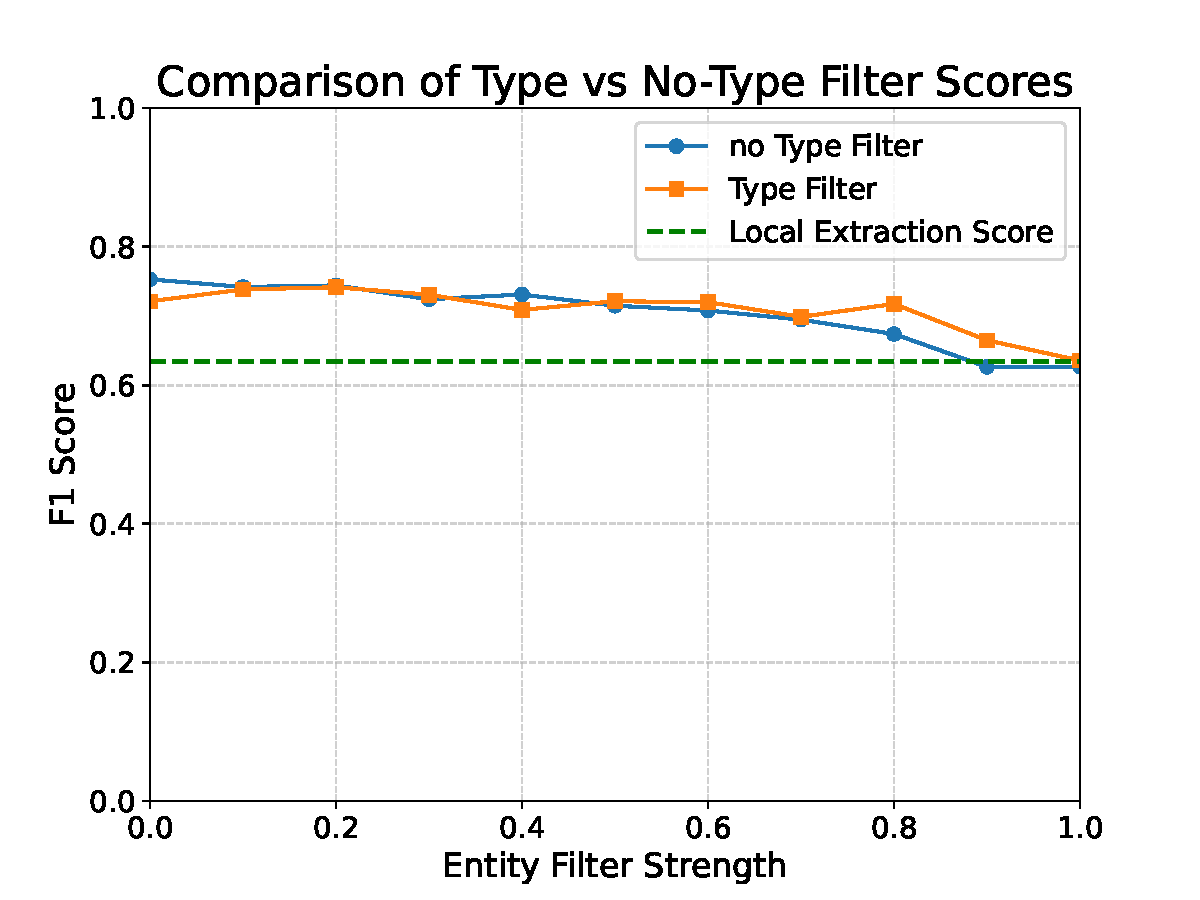
\includegraphics[width=\textwidth]{figures/c1_type_filter_scores.pdf}
        \caption{\textit{ROUGE-1 F1} across thresholds.}
        \label{approach-fig:type_filter_scores}
    \end{subfigure}
    \hfill
    \begin{subfigure}[b]{0.48\textwidth}
        \centering
        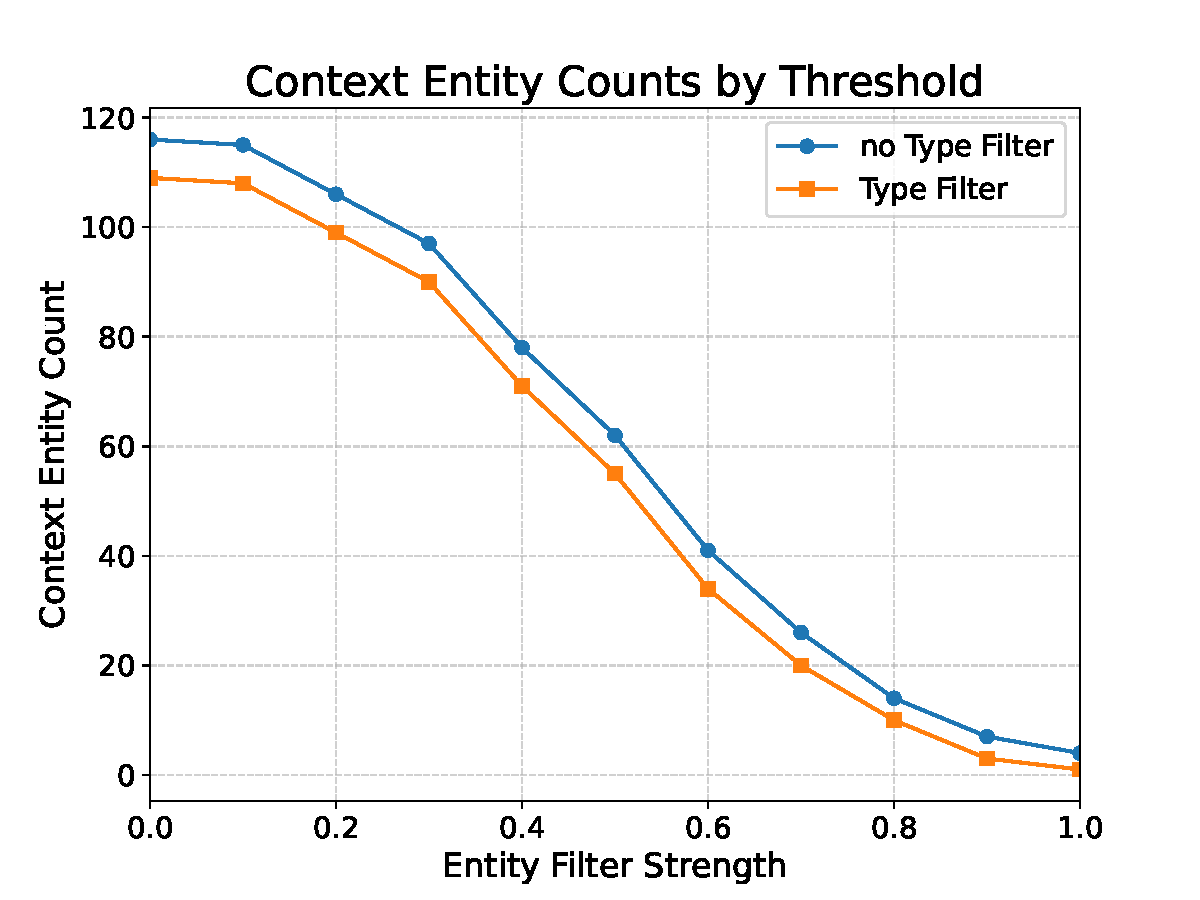
\includegraphics[width=\textwidth]{figures/c1_entity_counts.pdf}
        \caption{Entity counts across thresholds.}
        \label{approach-fig:entity_counts}
    \end{subfigure}
    \caption{Comparison of type-based and non-type-based filtering.
        (a) shows performance using \textit{ROUGE-1 F1} while (b) illustrates the corresponding entity counts.}
    \label{approach-fig:entity_filtering}
\end{figure}

Graph (a) shows that the \texttt{ENTITY\_FILTER\_STRENGTH} is inversely correlated with the extraction quality of the second extraction stage. Both lines (orange \& blue) stay consistent and start to drop off around 0.4. Regardless of the type-filter setting the extraction performance stays similar across all thresholds, indicating that the assumption made earlier (Section \ref{approach-subpar:type_filtering}) was correct. As a result we select $\texttt{ENTITY\_FILTER\_STRENGTH} < 0.4$ and activate filtering by entity type to further reduce the number of context entites.

Justification of the two-stage extraction can be found when comparing the green horizontal line (results after first extraction stage) with the results from the second extraction stage. The horizontal line consistently lies below the stage two results, only coming close when the filter removes almost all context-entities.

\subsubsection{Tuning: Graph Construction and Chain Risk}
We attempt to find the optimal parameters to extract all required \textit{document chains} which might be useful for reidentification. First, we measure the quality by comparing the number of connections between documents from the same cluster (intra-cluster connection) and documents from different clusters (inter-cluster connection). We aim to minimize inter-cluster connections while preserving most of the relevant intra-cluster connections.

The configurable parameter in this case is the \texttt{EDGE\_STRENGTH\_THRESHOLD}, which removes edges with too little strength. These are often inter-cluster connections, as documents about different topics typically share less entities. Removing these weak links
removes noise coming from many weak inter-cluster connections and therefore reduces the risk of false positives.
% prevents over-anonymization during the anonymization of entities. 
% For example: three documents \textit{doc1, doc2, doc3} form a chain, with strong links between \textit{doc1, doc2} but a single weak link to \textit{doc3}. If an entity is blurred in \textit{doc1, doc2} it will also be blurred in doc3, despite \textit{doc3} not being a risk, therefore potentially harming utility without improving privacy.

\begin{figure}[h]
    \centering
    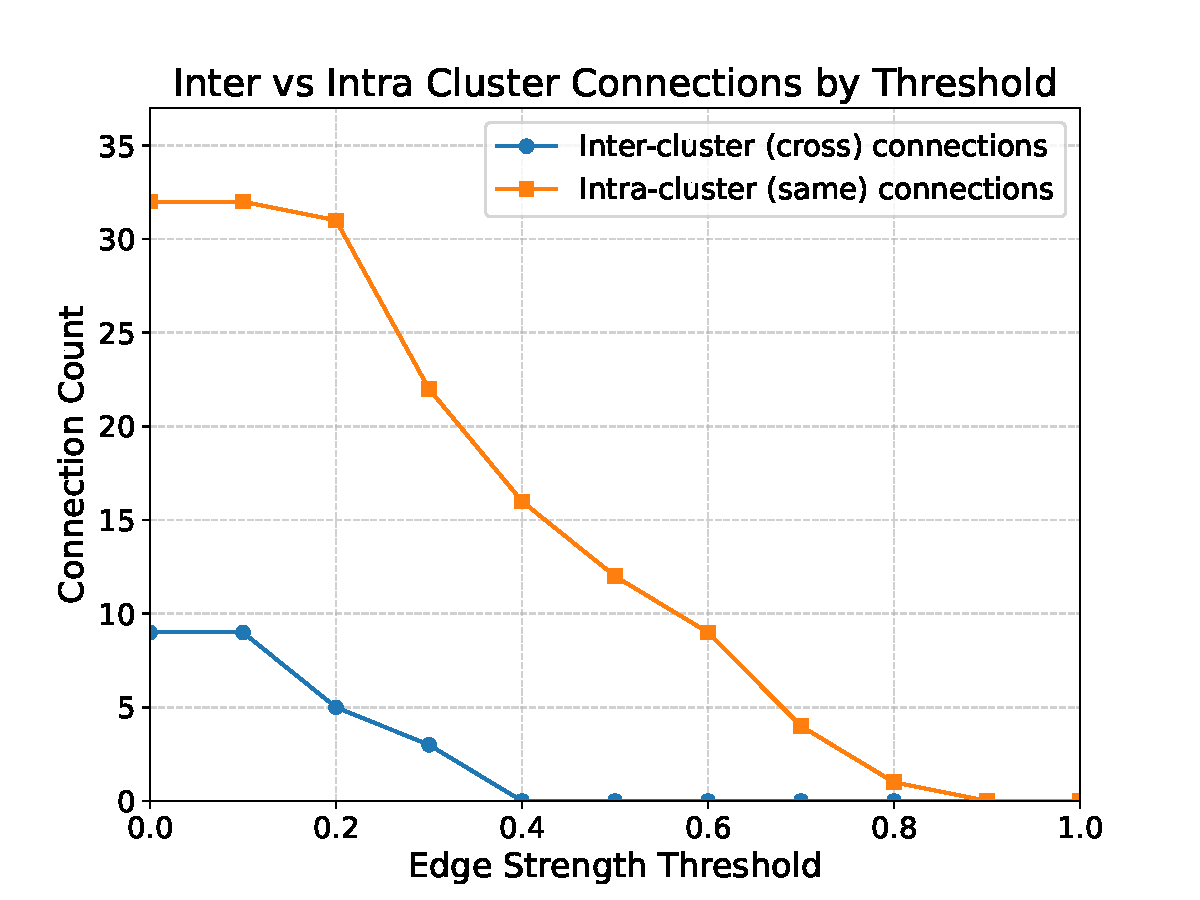
\includegraphics[width=0.7\textwidth]{figures/c2_cluster_connections_counts.pdf}
    \caption{Graph connections across \texttt{EDGE\_STRENGTH\_THRESHOLD}}
    \label{approach-fig:strength_connection_counts}
\end{figure}

For this train-dataset, a reasonable interval for the \texttt{EDGE\_STRENGTH\_THRESHOLD} is $[0.2,0.5]$. Within this interval a healthy number of intra-cluster connections remain, while inter-cluster connections drop steadily.

Using this interval as a starting point, we perform a grid-search including the surrounding intervals to find a final setting for the \texttt{EDGE\_STRENGTH\_THRESHOLD} and the optimal value for the \texttt{RISK\_THRESHOLD}. For simplicity we focus on the threshold defined for MEDIUM, as all \textit{document chains} above this threshold will be added as risks. We aim to find out whether the pipeline was able to identify and keep all relevant connections between documents up until this point. Our similarity measure is the F1-Score between all \textit{document chains} marked as dangerous by the pipeline and the hand-labeled \textit{document chains}.

\begin{figure}[h]
    \centering
    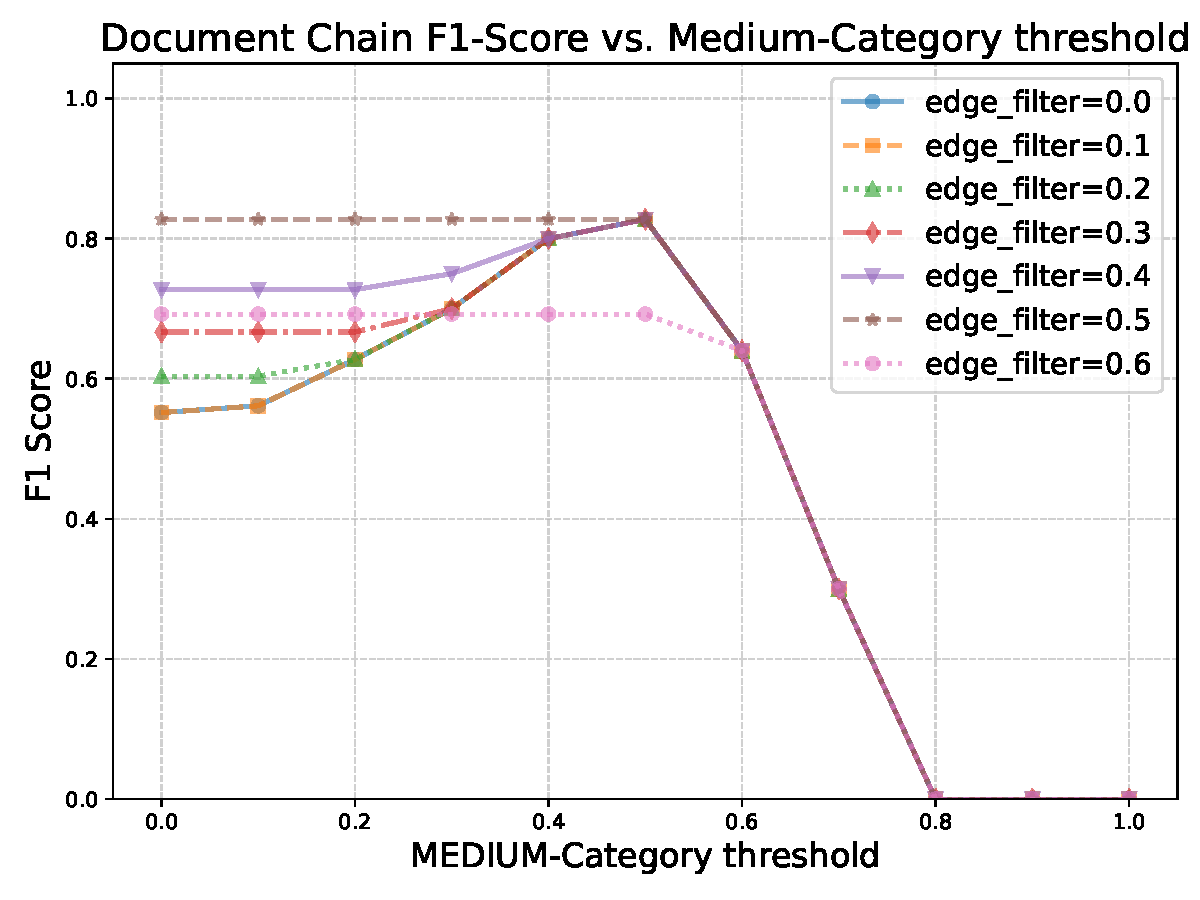
\includegraphics[width=0.7\textwidth]{figures/c2_f1_comparison.pdf}
    \caption{F1 Score for different combinations of \texttt{RISK\_THRESHOLD} and \texttt{EDGE\_STRENGTH\_THRESHOLD}}
    \label{approach-fig:f1_chain_score}
\end{figure}

Out of all different combinations, the setting: $\texttt{EDGE\_STRENGTH\_THRESHOLD} = 0.5$ performs the best, with a maximum F1-Score of $\approx 0.82$. The F1-Score is constant in the interval $\texttt{RISK\_THRESHOLD} \in [0.0,0.5]$, suggesting that for this example the pipeline didn't extract lower-risk chains which could be filtered out by setting $\texttt{RISK\_THRESHOLD}$ below $0.5$. Afterwards it begins to fall, indicating that relevant chains are being filtered out (see \ref{approach-fig:f1_chain_score}). We use this value as our final setting for the pipeline. The reported Recall and Precision can be found in the appendix () % TODO add reference to appendix and add two c2 graphs

\subsubsection{Tuning: Anonymization Thresholds}
The following section focusses on the the anonymization thresholds $\theta_{doc}$ and $\theta_{chain}$. We skip an extensive search for optimal $\rho_{risk\_level}$ as this relative reduction only acts as an additional safeguard.
Empirical testing indicate effective intervals of $\theta_{doc}\in[0.85,0.95]$ and $\theta_{chain}\in[0.4,0.6]$. Values below these intervals aggressively over-redacted even low-risk entities, while higher values had little effect due to overly lenient thresholds. Afterwards we performed a Grid Search over these intervals to find a suitable privacy-utility tradeoff using the benchmark proposed in Chapter \ref{chapter:evaluation}. Manual checks revealed unnecessary masking with $\theta_{doc}=0.85$, removing it as potential candiate value. As shown in Figure \ref{approach-fig:privacy_utility_thetas}, within the remaining combinations, $\theta_{doc}=0.95$ and $\theta_{chain}=0.50$ achieved the most favorable privacy-utility tradeoff: utility was substantially higher than at $\theta_{doc}=0.90$, with only a marginal loss in privacy. Therefore we adapt this setting as default.

It should be noted that due to the stochasticity of LLM-assisted evaluation and the limited dataset size, these hyperparameters should be regarded as strong empirical defaults rather than universally optimal settings.

\begin{figure}[h]
    \centering
    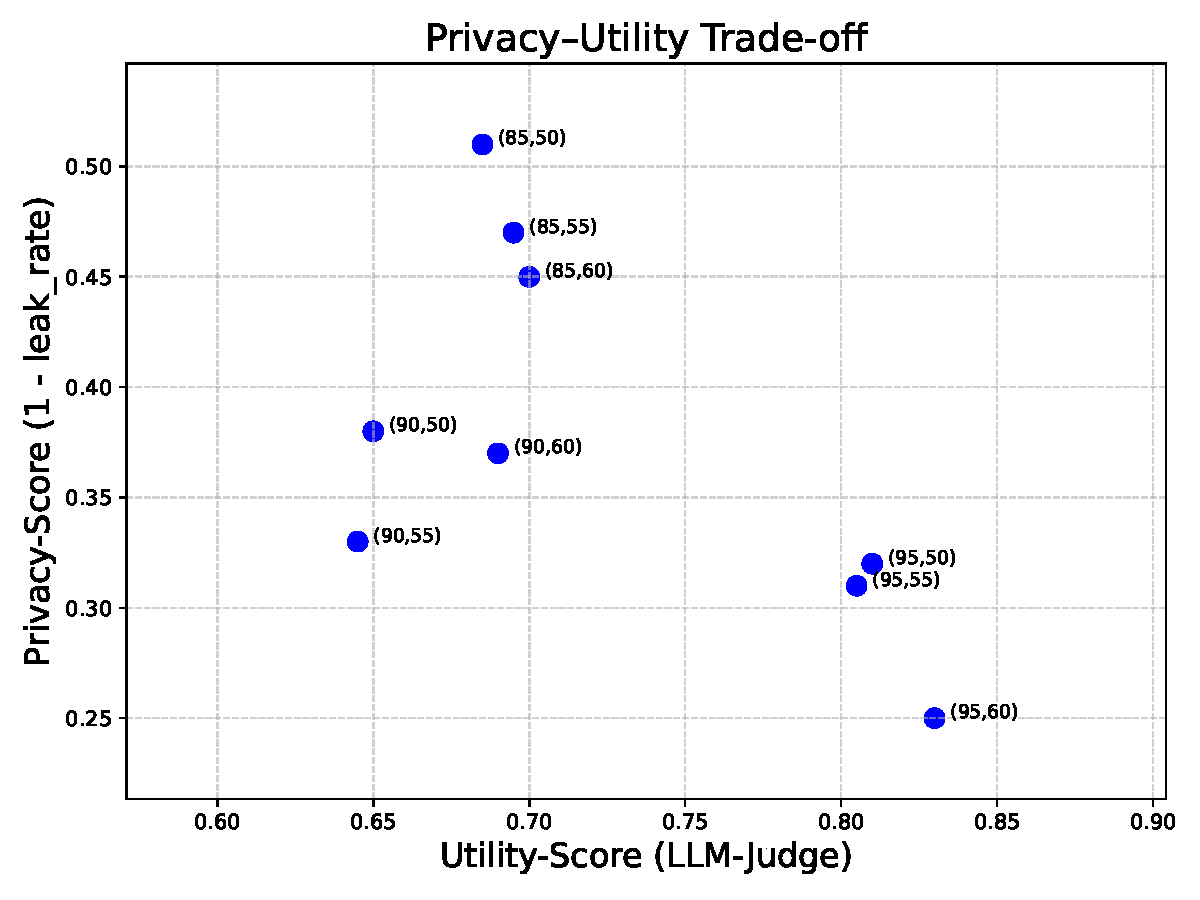
\includegraphics[width=0.7\textwidth]{figures/c3_privacy_utility_tradeoff.pdf}
    \caption{Privacy-Utility Tradeoff for different combinations for  $\theta_{doc}$ and $\theta_{chain}$ (higher is better)}
    \label{approach-fig:privacy_utility_thetas}
\end{figure}



% \begin{tikzpicture}[node distance=8mm and 12mm, font=/tiny, >=Latex] % Increased node distance slightly for clarity
%     \tikzset{
%         proc/.style={rectangle, rounded corners, draw, align=center, inner sep=3pt, fill=gray!5},
%         data/.style={rectangle, draw, align=center, inner sep=3pt, fill=blue!5},
%         dec/.style={diamond, draw, aspect=2, align=center, inner sep=1pt, fill=orange!10} % Not used, but kept for completeness
%     }

%     % --- First Column (Main Flow) ---
%     \node[data] (in) {JSON docs\\id, metadata, content};
%     \node[proc, below=of in] (norm) {Normalize text\\lowercase; document\_id=id||md5(content)};
%     \node[proc, below=of norm] (ext1) {Entity extraction I\\LLM per doc\\(original, normalized, type, relevance)};
%     \node[proc, below=of ext1] (filter) {Context filtering\\score=max\_rel$\cdot$uniqueness\\type filter, top-k};
%     \node[proc, below=of filter] (ext2) {Entity extraction II\\LLM with existing\_entities};

%     % --- Second Column (Parallel Flow 1: Risk Calculation) ---
%     % Position the first node of the second column to the right of the middle of the first column
%     \node[proc, right=of ext2] (uniq) {Uniqueness $u(e)$\\IDF-normalized over corpus};
%     \node[proc, below=of uniq] (riskd) {Document risk $R(d)=1-\prod(1-c_i)$\\$c_i=e_{rel}\cdot u(e)\cdot w_{type}$};
%         \node[proc, below=of riskd] (graph) {Document graph $G$\\edges on shared entities\\edge\_strength via $s_e$ and product};
%         \node[proc, below=of graph] (chains) {Chain analysis ($\leq k$) hop\\risk; $R_{chain}=1-\prod(1-hop)$\\categorize HIGH/MED/LOW};

%         % --- Third Column (Parallel Flow 2: Redaction) ---
%         % Position the first node of the third column to the right of the middle of the second column
%         \node[proc, below=of chains] (docred) {Doc-level redaction\\greedy by $s_e$=max\_d rel$\cdot$u$\cdot$w\\stop $R(d)<\theta_{doc}$};
%         \node[proc, below=of docred] (chainred) {Chain-level redaction\\greedy or knapsack by impact\\stop $R_{chain}\leq\theta_{chain}$ and $\rho$ rule};
%         \node[proc, below=of chainred] (replace) {Replacement\\value redaction [TYPE]\\or pseudonyms / redact / rewrite};
%         \node[data, below=of replace] (out) {Sanitized docs\\for indexing in RAG};


%         % --- Drawing Paths ---
%         % Main flow
%         \draw[->] (in) -- (norm);
%         \draw[->] (norm) -- (ext1);
%         \draw[->] (ext1) -- (filter);
%         \draw[->] (filter) -- (ext2);

%         % Connection from main flow to risk calculation
%         \draw[->] (ext2) -| (uniq); % Connects ext2 to uniq, then drops down

%         % Risk calculation flow
%         \draw[->] (uniq) -- (riskd);
%         \draw[->] (riskd) -- (graph);
%         \draw[->] (graph) -- (chains);

%         % Connection from risk calculation to redaction
%         \draw[->] (chains) -| (docred);

%         % Redaction flow
%         \draw[->] (docred) -- (chainred);
%         \draw[->] (chainred) -- (replace);
%         \draw[->] (replace) -- (out);

%         % Feedback loops (dashed lines) - Adjusted for new layout
%         \draw[<-, dashed] (docred.west) -| ($(uniq.south west)!0.5!(riskd.south west) - (1cm,0)$) |- (riskd.west);
%         \draw[<-, dashed] (chainred.west) -| ($(riskd.south west)!0.5!(graph.south west) - (1cm,0)$) |- (chains.west);


% \end{tikzpicture}

% In the document body

% !TeX root = ../main.tex
\chapter{Evaluation}\label{chapter:evaluation}
\section{Experimental Setup}
\section{RQ2: Does selective pseudonymization reduce privacy leakage on both the document and cross-document linkage level}
\section{RQ3: Does selective pseudonymization preserve higher utility compared to similar approaches}
% !TeX root = ../main.tex
\chapter{Discussion}\label{chapter:discussion}
\section{Ablation Studies}
In this section we discuss the different effects of parameters or algorithmic choices. An introductory study was already performed in Section \ref{approach-subsec:hyperparams} for the most relevant parameters. Here we focus more on the parameters that are not essential for the pipeline to function  but may be adjusted depending on the deployment context.  

All experiments are conducted on the same dataset used in the main evaluation. Variations of the sAnon configuration (Section \ref{evaluation-subsec:sanon-config}) are calculated using snapshots recorded during the initial evaluation. These snapshots capture the internal state of the pipeline immediately after entity extraction, eliminating non-determinism and ensuring stable and consistent comparisons.  Similar to the main evaluation we run each variation on three separate entity extractions and average the results to reduce noise.


\subsection{Varying chain lengths}
Increasing the chain length allows the graph to capture more long-range dependencies between documents, therefore potentially increasing the number of entities accumulated. This has different effects: (1) more entities increase the potential for reidentification, but (2) it also introduces noise which may lead to unwated redactions later. Table \ref{discussion-tab:chain_length} shows increasing chain length increases the number of redactions, thereby decreasing privacy leakage at a cost on downstream Q\&A. 

For this dataset our previous assumptions hold and $CL = 2$ achieves the best trade-off: moving from $CL=2$ to $CL=3$ yields a leakage reduction of $\approx 1\%$ but degrades average utility by $\approx 5.2\%$ for specific and by $\approx 7.3\%$ for general questions. Further increasing to $CL=4$ decreases privacy leakage by another $3.03\%$ with a marginal drop in utility (see Table \ref{discussion-tab:chain_length_percentage}).  We attribute this to our dataset's structure, where most relevant entity connections span only 2 documents.

In more complex corpora with longer inter-document dependencies, a higher $CL$ may perform better, but it will require careful context-dependent tuning to balance leakage reduction against utility loss.


\begin{table}[h!]
\centering
\caption{Summary for varying Chain Length (CL)}
\label{discussion-tab:chain_length}
\begin{tabular}{l c c c c}
\toprule
\textbf{ } & $CL = 2$ & $CL = 3$ & $CL = 4$ \\
\midrule
\# redacted entities & 245 & 260 & 283 \\
\midrule
privacy leakage & 0.634 &0.628 &0.609  \\
\midrule
specific / single & 0.421 & 0.389 & 0.386 \\
specific / multi & 0.278 & 0.270 & 0.266 \\
general / single & 0.784 & 0.765 & 0.764 \\
general / multi & 0.498 & 0.437 & 0.430 \\
\bottomrule
\end{tabular}
\end{table}

\begin{table}[h!]
\centering
\caption{Percentage-wise Comparison of Chain Lengths}
\label{discussion-tab:chain_length_percentage}
\begin{tabular}{l c c}
\toprule
\textbf{ } & CL=2 vs. CL=3& CL=3 vs. CL=4 \\
\midrule
\# redacted entities & +6.12\% & +8.85\% \\
\midrule

privacy leakage & -0.95\% & -3.03\% \\
\midrule
specific / single & -7.60\% & -0.77\% \\
specific / multi & -2.88\% & -1.48\% \\
general / single & -2.42\% & -0.13\% \\
general / multi & -12.25\% & -1.59\% \\
\bottomrule
\end{tabular}
\end{table}


\subsection{Document-level redaction only vs. full pipeline}
To justify the use of the proposed 2-stage redaction approach, we first isolate the effect of the document-level redaction. We compare the original pipeline with variants that only apply document-level redaction using thresholds $\theta_{doc}\in[0.8, 0.95]$. We then contrast these results with the full pipeline, combining document-level redaction followed by chain-level redaction. 

When comparing the effect of the full pipeline to the only-document-level redaction with $\theta_{doc} = 0.95$ in Table \ref{discussion-tab:theta_doc_llm}, we notice a drop in utility for specific questions while general-question utility is mostly preserved. 

\begin{table}[h!]
\centering
\caption{Summary for varying $\theta_{doc}$. KS is the Knapsack Algorithm here}
\label{discussion-tab:theta_doc_llm}
\begin{tabular}{l p{1.5cm} p{2cm} c c c c}
\toprule
\textbf{ } & \textbf{full pipeline} & $\theta_{doc} = 0.95$ {baseline}& $\theta_{doc} = 0.90$ &  $\theta_{doc} = 0.85$ & $\theta_{doc} = 0.80$\\
\midrule
\# redacted entities & 245 & 223 & 318 & 398 & 463  \\
\midrule
privacy leakage & 0.634 &0.669 &0.590 &0.531 &0.489  \\
\midrule
specific / single & 0.421 & 0.460 & 0.347 & 0.324 & 0.269 \\
specific / multi & 0.278 & 0.326 & 0.281 & 0.227 & 0.224  \\
general / single & 0.784 & 0.802 & 0.759 & 0.715 & 0.634  \\
general / multi & 0.498 & 0.532 & 0.459 & 0.449 & 0.448  \\

\bottomrule
\end{tabular}
\end{table}


To illustrate these differences, Table \ref{discussion-tab:percent-docOnly-Full} compares the percentage-wise reduction from $\theta_{doc} = 0.95$ to $\theta_{doc} = 0.90$ and the full pipeline. 

Analyzing the four utility categories reveals that the full pipeline consistently targets multi-source questions more than single source questions for both specific and general questions. In contrast, setting ($\theta_{doc} = 0.9$) yields a mixed pattern. Also, the second stage of the pipeline redacts specific-multi-source questions ($-14.72\%$) more than twice as much compared to general-multi-source questions ($-6.39\%$), confirming the expected \textit{selective-privacy effect}: patient-specific tasks requiring reasoning over documents are disproportionately targeted, while general-utility tasks retain relatively high performance.


Additionally the full pipeline appears to be more efficient: it reaches $\approx 44\%$ of the privacy improvement achieved by setting $\theta_{doc} = 0.90$, but requires only 22 instead of 95 entities to do so. A possible reason is the chain-risk scoring, which makes shared entities high-impact because masking them simultaneously lowers the edge strength and both endpoint document risks. This leads to the full pipeline being more surgical during entity redaction, therefore requiring less entities compared to the "blanket-redaction" performed by tightening $\theta_{doc} = 0.90$.

\begin{table}[h!]
\centering
\caption{Percentage change from the 0.95 $\theta_{doc}$ baseline}
\label{discussion-tab:percent-docOnly-Full}
\begin{tabular}{p{3.5cm} p{2cm} p{2cm} p{2cm} p{2cm}}
\toprule
\textbf{} & \textbf{specific/ single} & \textbf{specific/ multi} & \textbf{general/ single} & \textbf{general/ multi} \\
\midrule
\textbf{\% Change from 0.95 to Full (KS)} & -8.48\% & -14.72\% & -2.24\% & -6.39\% \\
\textbf{\% Change from 0.95 to 0.90} & -24.57\% & -13.80\% & -5.36\% & -13.72\% \\
\bottomrule
\end{tabular} 
\end{table}


% \subsection{Knapsack vs. Greedy}% TODO
% We expected a clearer separation between the algorithms with significantly fewer redaction and measurably higher performance by Knapsack (KS) when compared to Greedy selection. In our setting however, both methods reached the same privacy leakage, despite Knapsack redacting less entities. \footnote{The leakage rate was double checked and appears to be a coincidence}. 

% We attribute the similarity of both strategies to the small corpus (242 short documents). The benefits of using an optimal, minimal selection of entities for redaction likely becomes visible when the stronger linkage between more complex and longer documents is present. Under the current experiments scale, Greedy selection offeres a comparable privacy utility tradeoff, while KS yields slightly better multi-document general utility. 

% \begin{table}[h!]
% \centering
% \caption{Summary for Knapsack vs. Greedy Tradeoff}

% \label{discussion-tab:greedy_ks_llmjudge}
% \begin{tabular}{l c c c}
% \toprule
% \textbf{combination} & \textbf{sAnon\_Knapsack} & \textbf{sAnon\_Greedy}\\
% \midrule
% \# redacted entities & 245 & 248\\
% \midrule
% privacy leakage & 0.634 &0.634  \\
% \midrule
% specific / single & 0.421 & 0.433  \\
% specific / multi & 0.278 & 0.282  \\
% general / single & 0.784 & 0.785  \\
% general / multi & 0.498 & 0.464 \\

% \bottomrule
% \end{tabular}
% \end{table}


% \subsection{Value Redaction vs. Rewriting} % REMOVE probably
% When comparing 
% \begin{table}[h!]
% \centering
% \caption{Summary for Value Redaction vs. Rewriting}
% \label{discussion-tab:redact_rewrite_llmjudge}
% \begin{tabular}{l c c c}
% \toprule
% \textbf{combination} & \textbf{Value Redaction} & \textbf{Rewriting}\\
% \midrule
% privacy leakage & 0.568 &0.549 \\
% \midrule
% specific / single & 0.421 & 0.464  \\
% specific / multi & 0.278 & 0.269  \\
% general / single & 0.784 & 0.790  \\
% general / multi & 0.498 & 0.513 \\

% \bottomrule
% \end{tabular}
% \end{table}

% \subsection{Different extraction model choices}
%gpt20oss, gpt120oss, what else
% not ablation study, if needed put into separtaate section, but dont here


 
\section{Limitations}
While our pipeline achieves it's desired performance, it comes with many limitations, partially due to its strong dependency on the LLM-based entity extraction and normalization. Multi-word and overlappting entities can be inconsistently typed or split (e.g. "SF Potrero Hill Arthritis Center" as PROVIDER vs. LOCATION, where the shorter location span is also potentially needed for cross-document links) and normalization is not guaranteed across all appearing variations (e.g. "Dr Elise Varga" vs "Dr. Varga"). These effects are amplified by passing a long context during the second entity extraction pass, degrading overall performance.

% A potential mitigation worth exploring would be stricter prompting and more selective, similarity-based context passing.

Due to the methods heuristic approach of quantifying risks, it requires careful \& extensive tuning of hyperparameters to achieve it's maximal potential and is unable to provide formal guarantess (unlike Differential Privacy approaches). 


Regarding the synthetic benchmark: it controls overlap and risk within documents and clusters but is unable to simulate messy real-world data or structured artifacts (e.g., benign tables) that might lead to  unwarranted redaction.



presentation first week of october


	
% !TeX root = ../main.tex
\chapter{Conclusion}\label{chapter:conclusion}
ff



%%
%% The next two lines define the bibliography style to be used, and
%% the bibliography file.
\bibliographystyle{ACM-Reference-Format}
\bibliography{bibliography}


%%
%% If your work has an appendix, this is the place to put it.
\appendix
\appendix

\chapter{Appendix: Approach}
\section*{Extraction Prompt Templates}
\subsection*{Local Entity Extraction Prompt}

his


\chapter{Appendix: Experimental Setup \& Data Generation}
\section*{Prompt Templates}
\subsection*{Standard RAG Query Template}\label{appendixB:std-rag-template}
\begin{tcolorbox}[title=Standard RAG Query]
Answer the question based on only the following context:\\\\
\{context\}\\\\
---\\\\
Question: \{query\}\\\\
Answer:
\end{tcolorbox}

\pagebreak

\subsection*{Data Generation Templates}
\subsubsection*{Expected JSON schema for cluster generation}

\begin{lstlisting}[language=json,caption={Expected output JSON schema for cluster generation},label={appendixB:json-schema-generation}]
{
  "documents": [
    {
      "id": "cluster_{cluster_id}_doc{doc_index}",
      "content": "string (40-120 words realistic text)",
      "metadata": {
        "format": "claim_form|medical_record|insurance_memo|provider_report|patient_survey|research_note|policy_document|audit_report|news_article"
      }
    }
    // additional documents ...
  ],
  "metadata": {
    "category": "cluster",
    "cluster_id": "string",
    "cluster_risk": "HIGH|MEDIUM|LOW",
    "content_summary": "string (brief summary)",
    "person": {
      "entities": [
        ["entity value", "entity type"], ...
      ]
    },
    "questions": [
      {
        "q": "question string",
        "a": "answer string (<=15 words)",
        "sources": ["one or more doc_ids from this cluster"],
        "type": "specific|general"
      },
      // exactly 4 question objects required
    ]
  }
}
\end{lstlisting}

\subsubsection*{Cluster generation prompts}\label{appendixB:cluster-gen-prompts}
The Output JSON Schema has been omitted for brevity reasons. See Listing \ref{appendixB:json-schema-generation} for details.

\begin{tcolorbox}[title={System prompt - Cluster generation }]
\footnotesize
\begin{lstlisting}[breaklines=true, label={appendixB:sys-cluster-prompt}]
You are an advanced synthetic health insurance document cluster generator specifically designed to test privacy-preserving RAG systems. 

Return ONE valid JSON object only-no prose, no code fences.

SCHEMA (required keys & types):
// refer to previous section for Schema
---

GENERATION RULES

1. Entity Strategic Placement
- Use only allowed_types: {allowed_types}
- Place "anchor" entities (e.g. dates, locations, procedures, IDs) that connect documents.
- Include identifying combinations of common entities that become unique together

2. Advanced Person Modeling
- Each cluster represents ONE complex individual across multiple touchpoints
- Design multi-faceted personas with overlapping institutional interactions
- Allow temporal progression (e.g., care journey, claims timeline) or edge cases (rare conditions, unusual circumstances, outlier demographics)
- Documents containing information about the individual MUST BE LINKED in some way (shared entity, location, etc.)!

3. Sophisticated Risk Profiles regarding modeled person
- HIGH: >=7 entities, >=3 critical/high vulnerability, 70-90% cross-document overlap, unique combinations, person identifiable through little to no document linking
- MEDIUM: 4-6 entities, <=2 critical, 40-60% overlap, some rare elements, person identifiable through extensive document linking
- LOW: <=4 entities, mostly low vulnerability, <=30% overlap, person not identifiable through document linking

4. Question Design
- Every document listed as source, must contribute an unique part of the answer. 
- Answers must be <=15 words, factual, and self-contained to the cluster (no external knowledge required)
- Questions must have high similarity with their sources to allow standard RAG to retrieve them properly
- type: specific
    - person-focused
    - clear reference to the person or rare/unusual combinations (e.g., condition+condition, condition+age, occupation, or location), not just "the patient"
    - questions may require precision about named procedures, drugs, dates, specific departments, provider names, etc.
    - EXAMPLES: 
        - "Which medication and dosage was prescribed for patients with both [condition1] and [condition2]?"
        - "Which two specialists did patient [patient_id] visit?"
- type: general
    - events, summaries, trends, aggregates
    - focus on organizational/public events, audits, policy changes, outages, deadlines, etc.
    - Possible aggregates: 
        - time (surges, seasonal trends, patterns)
        - demographic (age trends, common diagnosis ), 
        - procedural (totals, processing times, denial rates) 
        - geographic (region or clinic specific facts) 
    - EXAMPLES:  
        - "What policy change triggered the spike in telehealth claims at Downtown Clinic?" 
        - "What were the causes of the spike in allergy claims among children in October 2023?"
        - "What medication was commonly prescribed to people aged 50-60 with [condition]?"
        - "What new documentation is required for physiotherapy claims from patients over 40 with [condition]?"
- sources: single == 1 source, multi >= 2 sources

5. Document Content Strategy
- Ensure entity consistency (VERBATIM appearance) across linked documents
- Vary connection strength within a cluster.
- Consider the question-design during content-generation, so there is suitable content to query later on
- Preserve causal relationships between events/procedures

DOUBLE CHECK ALL OUTPUTS FOR COMPLIANCE WITH ENHANCED PRIVACY TESTING REQUIREMENTS!
\end{lstlisting}
\end{tcolorbox}

\pagebreak
\begin{tcolorbox}[title={User prompt template - Cluster generation}]
\footnotesize
\begin{lstlisting}[breaklines=true,label={appendixB:user-cluster-prompt}]
Create one sophisticated health insurance cluster (risk={cluster_risk}) designed to test privacy-preserving RAG systems:

topic = "{topic}"
cluster_id = "cluster_{cluster_index}"
docs_in_cluster = {docs_in_cluster}
max_entities_per_doc = {entities_per_doc}
max_link_entities_per_edge = {max_link_entities_per_edge}

DIVERSITY CONSTRAINTS:
- Avoid these used medical conditions: {used_conditions}
- Avoid overusing these locations: {used_locations}  
- Avoid overusing these demographics: {used_demographics}
- Don't repeat these scenarios: {history_summary}

IMPORTANT RULES:
- Do not mark the placed entities in any way (DO NOT DO THE FOLLOWING: "the patient was AGE 56 and had MEDICAL_CONDITION prion-disease")
- Create exactly 4 questions with the following (type, sources) combination: (single, specific) (single, general) (multi, specific) (multi, general)
- There are many other clusters, keep the questions unique, specific and linkable to the current cluster
    - always add some identifying entity to link the questions to the documents (e.g. location, policy number, time)
    - don't ask about "this patient", "a policy", etc. if there is no other linking entity present in the question
- use realistic sounding entities (no Jane Doe, Springfield, etc.)

Return ONLY JSON matching the enhanced schema.
Allowed entity types: {allowed_types}
Forbidden entity types: {forbidden_types}
\end{lstlisting}
\end{tcolorbox}


\pagebreak
\subsubsection*{Cluster refinement prompts}\label{appendixB:cluster-refine-prompts}

\begin{tcolorbox}[title={System prompt template - Entity refinement}]
\footnotesize
\begin{lstlisting}[breaklines=true]
You are an entity extractor for health data, focused on identifying entities belonging to a specific person in documents. 

Given a set of documents and an initial list of person entities, re-evaluate and extract all entities that belong to the specific person hidden in the current documents. Use only the allowed entity types.

Output ONLY a valid JSON object with the key "entities" containing the updated list: 
{{
  "entities": [
    ["entity value", "entity type from allowed_types"]
  ]
}}

- Ensure the output is strictly a JSON object.
- Entities must be unique and verbatim from the documents.
- Focus exclusively on entities that identify or relate to the single person modeled in the cluster.
- Allowed entity types: {allowed_types}
- If no entities are found, return an empty list.
\end{lstlisting}
\end{tcolorbox}

\begin{tcolorbox}[title={User prompt template - Entity refinement}]
\footnotesize
\begin{lstlisting}[breaklines=true]
Documents:
{documents_json}

Current person entities:
{current_entities_json}

Re-evaluate and provide an updated "entities" list based on all entities belonging to the specific person in these documents. Output only the JSON object.
\end{lstlisting}
\end{tcolorbox}


\pagebreak
\begin{tcolorbox}[title={System prompt template - Question refinement}]
\footnotesize
\begin{lstlisting}[breaklines=true]
You are a question-auditor for synthetic health-insurance clusters.
Verify four Q-A pairs and edit only when needed so each strictly follows all rules.

1. Source necessity
- Every listed doc-id must be essential to answer the question.  
- If a multi-source pair only requires one source, rewrite per Rule 3 so at least 2 docs are indispensable.

2. Preserve metadata
- Keep the question count (4).  
- Keep each pair's "type" value (specific | general).  
- Maintain single/multi status after auditing:  
  - single = exactly 1 source  
  - multi  = at least 2 sources

3. Editing (preferred)
- Rewrite the question or answer minimally to satisfy rules.  
- Allowed changes:  
  - Adjust question, answer and sources or replace the question (see Rule 4).  
  - Improve question wording if retrieval via RAG would be hard.

4. Replacing a question
- Mirror wording in the sources.  
- "Specific" = person-focused, rare entity combos (e.g. ID, age, condition, location).  
- "General" = events, summaries, trends, aggregates.  
- Each source must supply unique information; omitting one makes the answer impossible.  
- Answer <= 15 words; no external knowledge beyond sources.

OUTPUT  
Return ONLY:
{{
  "questions": [
    {{
      "q": "possibly modified question",
      "a": "unchanged or updated answer",
      "sources": ["doc-id", ...],
      "type": "specific|general"
    }}
    /* exactly four such objects */
  ]
}}
\end{lstlisting}
\end{tcolorbox}


\begin{tcolorbox}[title={User prompt template - Question refinement}]
\footnotesize
\begin{lstlisting}[breaklines=true]
    Current questions JSON:
    {questions_json}

    Cluster documents JSON:
    {documents_json}

    Verify / prune sources and, if required, update each question or answer text
    so the remaining sources are strictly necessary.  Follow the rules.
\end{lstlisting}
\end{tcolorbox}

\subsection*{SAGE Prompt Templates}\label{appendixB:sage-prompts}
Only the most important prompts and snippets are listed here. A detailed list of all prompts used for both stages can be found on % TODO add github link after polishing SAGE implementaion
\begin{tcolorbox}[title={Stage 1: Synthetic data generation}]
\footnotesize
\begin{lstlisting}[breaklines=true, label={appendixB:synth-datagen-prompt}]
You are generating a synthetic {doc_format} document based on the following extracted key information. 

The synthetic document should:
1. Maintain the essential information and context from the key attributes
2. Be approximately {original_length} characters in length
3. Follow the typical format and style of a {doc_format}


Key Information to Preserve:
{info_text}

Generate a synthetic document that incorporates this key information. Make sure the document reads naturally and maintains professional language appropriate for a {doc_format}.

Return your response in the following JSON format:
{{
    "synthetic_content": "synthetic content"
}}
\end{lstlisting}
\end{tcolorbox}

\begin{tcolorbox}[title={Stage 2: Privacy agent snippet}]
\footnotesize
\begin{lstlisting}[breaklines=true, label={appendixB:priv-agent-prompt}]
You are a privacy assessment expert. Your task is to analyze a synthetic document for potential privacy issues compared to its original version.

Original Document:
{original_content}

Synthetic Document:
{synthetic_content}

Analyze the synthetic document for the following privacy concerns only regarding patient or clamaint identification:

// the rules regarding privacy have been omitted to avoid clutter

Return your assessment in the following JSON format:
{{
    "safe": true/false,
    "suggestions": [
        "List any privacy concerns and specific suggestions for improvement if issues found"
    ]
}}

Only if the generated data is completely safe and satisfies all the above privacy requirements and prevents the recovery of the original data, set "is_safe": true and leave issues/suggestions empty.
\end{lstlisting}
\end{tcolorbox}

\begin{tcolorbox}[title={Stage 2: Rewriting agent snippet}]
\footnotesize
\begin{lstlisting}[breaklines=true, label={appendixB:rewriting-agent-prompt}]
You are a document rewriting expert. You need to improve the following synthetic document based on privacy feedback.

Current Synthetic Document:
{synthetic_content}

Suggestions for improving privacy issues:  
{suggestions}

Please rewrite the document to address these privacy concerns while maintaining:
1. the essential information and context of the original
2. high utility and is privacy preserving
3. the appropriate professional tone and format

Return your response in the following JSON format:
{{
    "rewritten_content": "rewritten content"
}}
\end{lstlisting}
\end{tcolorbox}

\

\subsection*{LLM Judge Prompts}\label{appendixB:llm-judge-prompts}

\begin{tcolorbox}[title={LLM-Judge: Answer quality prompt}]
\footnotesize
\begin{lstlisting}[breaklines=true, label={appendixB:llm-judge-answer-quality}]
Evaluate the quality of the RAG System Answer compared to the Expected Answer. Rate the answer on a scale from 0.0 to 1.0 (higher equals better).
        
Question: {q.question}
Expected Answer: {q.optim_answer}
RAG System Answer: {rag_answer}
Question Type: {"Multi-document" if q.origin == "multi" else "Single-document"}

Evaluation Criteria:
- Completeness of information
- Factual accuracy compared to expected answer

RESPOND WITH ONLY THE FOLLOWING SCHEMA! ONLY RESPOND WITH VALID JSON:
{{ "score": number }}
\end{lstlisting}
\end{tcolorbox}

\begin{tcolorbox}[title={LLM-Judge: Entity-leakage detection prompt}]
\footnotesize
\begin{lstlisting}[breaklines=true, label={appendixB:llm-judge-leakage}]
Accumulated RAG System answer: {rag_answer}

Which of the following entities also appears in the accumulated RAG System answer?
person_entities: [{', '.join(e[0] for e in person.entities)}].

An entity can appear verbatim, in a normalized form (e.g. different date format) or be easily inferrable from the answer.

Do not output the verbatim value of the appearing entity from the text, but the value from person_entities you have matched it to!

RESPOND WITH ONLY THE FOLLOWING SCHEMA! ONLY RESPOND WITH VALID JSON:
{{ "leaked_entities": [list of leaked entities that also appear in person.entities] }}
\end{lstlisting}
\end{tcolorbox}

\section*{Miscellaneous}
\subsection*{Data Generation RISK-level specifications}\label{appendixB:risk-specifications}
\begin{table}[h]
\centering
\caption{Entity-type allowance by \texttt{RISK} level}
\label{appendixB:risk-specification-entity-matrix}
\renewcommand{\arraystretch}{1.1}
\begin{tabular}{|l|c|c|c|}
\hline
\textbf{Entity type} & \texttt{HIGH} & \texttt{MEDIUM} & \texttt{LOW} \\
\hline
NAME                 & x &   &   \\
EMAIL                & x & x &   \\
PHONE\_NUMBER        & x & x &   \\
ADDRESS              & x & x &   \\
PATIENT\_ID          & x & x &   \\
NON\_PERSONAL\_ID    & x & x & x \\
BIRTHDATE            & x & x & x \\
AGE                  & x & x & x \\
UNIQUE\_FACT         & x & x & x \\
INDIRECT\_IDENTIFIER & x & x & x \\
MEDICAL\_CONDITION   & x & x & x \\
EVENT\_DATE          & x & x & x \\
LOCATION             & x & x & x \\
DEMOGRAPHIC          & x & x & x \\
EVENT                & x & x & x \\
PROVIDER             & x & x & x \\
TREATMENT            & x & x & x \\
\hline
\end{tabular}
\end{table}


\subsection*{Experiments: Entity Leakage per Type}\label{appendixB:entity-leak-per-type}
This table compares the number of leaked entities for all baselines. Potential errors due to regex-filtering failing for targeted attacks, leading to false positives. 
\begin{table}[h!]
\centering
\caption{Leakage by type for each baseline}
\label{evaluation-tab:type_leakage}
\begin{tabular}{l c c c c}
\toprule
\textbf{entity\_type} & \textbf{total number} & \textbf{std\_RAG} & \textbf{sAnon} & \textbf{SAGE} \\
\midrule
ADDRESS & 11 & 11 & 2 & 0 \\
AGE & 20 & 20 & 15 & 9 \\
BIRTHDATE & 18 & 17 & 1 & 0 \\
DEMOGRAPHIC & 18 & 18 & 17 & 10 \\
EMAIL & 5 & 2 & 2 & 0 \\
EVENT & 17 & 12 & 14 & 9 \\
EVENT\_DATE & 72 & 58 & 42 & 37 \\
INDIRECT\_IDENTIFIER & 10 & 9 & 7 & 4 \\
LOCATION & 34 & 33 & 29 & 22 \\
MEDICAL\_CONDITION & 68 & 66 & 38 & 48 \\
NAME & 12 & 12 & 0 & 0 \\
NON\_PERSONAL\_ID & 36 & 31 & 9 & 14 \\
PATIENT\_ID & 41 & 39 & 0 & 1 \\
PHONE\_NUMBER & 1 & 1 & 1 & 0 \\
PROVIDER & 41 & 35 & 33 & 11 \\
TREATMENT & 119 & 116 & 103 & 91 \\
UNIQUE\_FACT & 46 & 42 & 40 & 17 \\
\bottomrule
\end{tabular}
\end{table}






\end{document}
\endinput
%%
%% End of file `sample-sigconf.tex'.
